\documentclass[conference]{IEEEtran}
\IEEEoverridecommandlockouts
% The preceding line is only needed to identify funding in the first footnote. If that is unneeded, please comment it out.
\usepackage{braket}
\usepackage{comment}
\usepackage{cite}
\usepackage{amsmath,amssymb,amsfonts}
\usepackage{algorithmic}
\usepackage{graphicx}
\usepackage{textcomp}
\usepackage{xcolor}
\def\BibTeX{{\rm B\kern-.05em{\sc i\kern-.025em b}\kern-.08em
    T\kern-.1667em\lower.7ex\hbox{E}\kern-.125emX}}
\begin{document}

\title{Quantum Algorithm for Linear Systems of Equations\\
}

\author{\IEEEauthorblockN{Alfred Nguyen}
\IEEEauthorblockA{\textit{Department of Computer Science} \\
\textit{Technical University of Munich} \\
85748 Garching, Bavaria\\
alfred.nguyen@outlook.com}
}

\maketitle

%%%%%%%%%%%
% Subsections
%%%%%%%%%%%
% 
\begin{abstract}
This document is a model and instructions for \LaTeX.
This and the IEEEtran.cls file define the components of your paper [title, text, heads, etc.]. *CRITICAL: Do Not Use Symbols, Special Characters, Footnotes, 
or Math in Paper Title or Abstract.
\end{abstract}

\begin{IEEEkeywords}
component, formatting, style, styling, insert
\end{IEEEkeywords}




\section{Ease of Use}

\subsection{Maintaining the Integrity of the Specifications}

The IEEEtran class file is used to format your paper and style the text. All margins, 
column widths, line spaces, and text fonts are prescribed; please do not 
alter them. You may note peculiarities. For example, the head margin
measures proportionately more than is customary. This measurement 
and others are deliberate, using specifications that anticipate your paper 
as one part of the entire proceedings, and not as an independent document. 
Please do not revise any of the current designations.

\section{Prepare Your Paper Before Styling}
Before you begin to format your paper, first write and save the content as a 
separate text file. Complete all content and organizational editing before 
proofreading, spelling and grammar.

Keep your text and graphic files separate until after the text has been 
formatted and styled. Do not number text heads---{\LaTeX} will do that 
for you.

\subsection{Abbreviations and Acronyms}\label{AA}
Define abbreviations and acronyms the first time they are used in the text, 
even after they have been defined in the abstract. Abbreviations such as 
IEEE, SI, MKS, CGS, ac, dc, and rms do not have to be defined. Do not use 
abbreviations in the title or heads unless they are unavoidable.

\subsection{Units}
\begin{itemize}
\item Use either SI (MKS) or CGS as primary units. (SI units are encouraged.) English units may be used as secondary units (in parentheses). An exception would be the use of English units as identifiers in trade, such as ``3.5-inch disk drive''.
\item Avoid combining SI and CGS units, such as current in amperes and magnetic field in oersteds. This often leads to confusion because equations do not balance dimensionally. If you must use mixed units, clearly state the units for each quantity that you use in an equation.
\item Do not mix complete spellings and abbreviations of units: ``Wb/m\textsuperscript{2}'' or ``webers per square meter'', not ``webers/m\textsuperscript{2}''. Spell out units when they appear in text: ``. . . a few henries'', not ``. . . a few H''.
\item Use a zero before decimal points: ``0.25'', not ``.25''. Use ``cm\textsuperscript{3}'', not ``cc''.)
\end{itemize}

\subsection{Equations}
Number equations consecutively. To make your 
equations more compact, you may use the solidus (~/~), the exp function, or 
appropriate exponents. Italicize Roman symbols for quantities and variables, 
but not Greek symbols. Use a long dash rather than a hyphen for a minus 
sign. Punctuate equations with commas or periods when they are part of a 
sentence, as in:
\begin{equation}
a+b=\gamma\label{eq}
\end{equation}

Be sure that the 
symbols in your equation have been defined before or immediately following 

\subsection{\LaTeX-Specific Advice}

Please use ``soft'' (e.g., \verb|\eqref{Eq}|) cross references instead
of ``hard'' references (e.g., \verb|(1)|). That will make it possible
to combine sections, add equations, or change the order of figures or
citations without having to go through the file line by line.

Please don't use the \verb|{eqnarray}| equation environment. Use
\verb|{align}| or \verb|{IEEEeqnarray}| instead. The \verb|{eqnarray}|
environment leaves unsightly spaces around relation symbols.



\section{Template}




Please note that the \verb|{subequations}| environment in {\LaTeX}
will increment the main equation counter even when there are no
equation numbers displayed. If you forget that, you might write an
article in which the equation numbers skip from (17) to (20), causing
the copy editors to wonder if you've discovered a new method of
counting.

{\BibTeX} does not work by magic. It doesn't get the bibliographic
data from thin air but from .bib files. If you use {\BibTeX} to produce a
bibliography you must send the .bib files. 




\begin{abstract}
Linear systems are a fundamental problem in math or can be found in subroutines in more complex tasks.
Linear systems are in the form of $A \vec x = \vec b$, where $A$ is a given matrix, $\vec b$ is a given vector and $\vec x$ is the unknown to be solved.
The HHL (Harrow, Hassidim, and Lloyd) algorithm is a quantum algorithm, that is able to solve these linear systems of equations exponentially faster than its classical counter part. 
Though, there are a few caveats to consider.
We assume that we only want to solve for an expectation value of some operator on $\vec x$, e.g. $\vec{x}^\dagger M \vec x$ for some matrix $M$.
That means we are not interested in the whole solution of $\vec x$.
Also, we assume that the matrix $A$ is sparse and is in the size of $N\times N$. 
Given these requirements, classical algorithms can solve this problem in $\mathcal{O}(N )$, whereas the HHL algorithm can solve this problem in $\mathcal{O}(log (N) )$.
This gives us an exponential speedup over the classical method.
\end{abstract}

\begin{IEEEkeywords}
Harrow-Hassidim-Lloyd (HHL) quantum algorithm, 
Quantum Fourier transform (QFT), 
Inverse Quantum Fourier transform (IQFT), 
Quantum Phase Estimation (QPE),
is that everything?
\end{IEEEkeywords}



\section{Introduction}


Quantum computing has a lot of potential in many various domains. 
It leverages the power of quantum superposition and entanglement to perform computations that a classical compuer cannot similate.
In some cases, quantum computer algorithms can provide an exponential speed up in comparison to common classical methods.
The most famous case being the Shor's algorithm for factoring large numbers, possibly cracking our current RSA encryption.

Solving linear systems is a fundamental subproblem in many scientific, engineering and mathematical discplines. 
Currently, the demand for processing data sets is increasing. 
The sizes of these datasets which make up the equations, is growing well into terabytes and petabytes of data.
Obtaining solutions for these kind of problems can be very computational expensive.
Even an approximation of these solutions with $N$ unknowns take at least $N$ timesteps.
Just outputting the solution takes at least N steps, as we have to read out all the $N$ unkowns for the whole solution.

Though, oftentimes we are not interestd in the full solution vector. 
For example, we can assume that we are only interested in a function, that determines the weights of some subsets in a specific region of the vector.
Then we can achieve an exponential faster approximation by using quantum computers. 
In the end we will observe, that the sparsity and conditioning of the problem matrices $A$, have comparable dependency on the runtime, but the error dependency is exponentially worse. 

Especially in quantum machine learning these kind of problems arise very frequently. 
Using large datasets finding patterns, classifying and clustering are very common methods which demand a lot of resources. 
Many of the quantum machine learning algorithms extend or use the following algorithm as a subroutine. 

This paper will focus on an algorithm, which can estimate features of the solution vector of a linear system of equations.
The HHL algorithm, designed by Aram Harrow, Avinatan Hassidim and Seth Lloyd, was introduced in 2009. 
It is one of the groundbreaking algorithms in quantum computing alongside Shor's factoring algorithm, Grover's search algorithm, and the quantum fourier transform (QFT).
Given an $N \times N$ sparse matrix $A$, the HHL algorithm runs in $\mathcal{O} (log (N))$, whilst the classical counterpart runs in $\mathcal{O} (N)$.
This promises us an exponential speed up over the commonly used classical method.

\subsubsection{Outline}
Firstly, this paper will give a rough overview of the HHL algorithm, specifying the problem in detail, giving a mathematical idea of the algorithm, followed by the explanation of the quantum circuit.
Then, we will discuss the HHL algorithm, going through all the phases of the algorithm.
Next, we evaluate and analyze its runtime by comparing the HHL algorithm by its classical counterpart. 
Afterwards, we will take an outlook at future works, exploring potential applications, variations of the HHL algorithm and will relate it to IT security. 
In the end we will give a final conclusion, summarizing our findings. 




\begin{comment}
    
Considering these constraints can be useful
where N is large spares and condition is small 

Quick walkthrough of the algorithm

main part is the QPE
encoding vector into quantum state


Physical drawback?

Quantum technologies face inherent noise and errors due to factors such as decoherence and imperfect gate operations. 
Additionally, the HHL algorithm requires high precision and control over quantum operations, making it particularly sensitive to these errors. 
As a result, the algorithm is currently more suited for small-scale problem instances and specialized applications.

Nonetheless, the HHL algorithm has generated significant interest and research efforts in the quantum computing community. 
Its potential impact spans various fields, including optimization, machine learning, cryptography, and simulation. 
As quantum technologies continue to advance and overcome the current limitations, the HHL algorithm holds the promise of revolutionizing the field of linear systems solving and contributing to the broader quest for harnessing the power of quantum computing to tackle complex computational problems.
\end{comment}
\section{Quantum computing concepts}
In this section, we will define common quantum computing concepts, relevant for understanding the HHL algorithm.

\subsection{Bra-ket Notation}
The \textit{bra-ket} notation is commonly used to represent quantum states, operators and measurements.
To begin with, a qubit can be represented by a 2d-vector $\vec v$ which can be written in its \textit{ket} form $\ket v$.
The most common \textit{kets} are the $0$ and $1$ \textit{kets}, which are written as $\ket 0$ and $\ket 1$ respectively.
These are the basis states that represent the 0 and 1 bit on a classical computer. 
As already mentionend, we can think of a \textit{ket} as a vector. 
In vector form $\ket 0$ and $\ket 1$ are the defined by these vectors as such

\begin{equation}
  \ket 0  = \begin{pmatrix}1\\0\end{pmatrix} 
\end{equation}

\begin{equation}
  \ket 1  = \begin{pmatrix}0\\1\end{pmatrix}
\end{equation}

Graphically we can think of these two qubits $\ket 0$ and $\ket 1$ as two orthonormal vectors one pointing upwards and the other to the right, whilst having the length of 1.

Multiple qubits can be combined to a quantum state often refered to as $\ket \Psi$, describing the state of a quantum computer. 
For example, if we have a quantum computer with 4 qubits which are all initialized to the 0 state, where the state $\ket \Psi$ would look as such

\begin{equation}
    \ket \Psi = \ket 0 \otimes \ket 0 \otimes \ket 0 \otimes \ket 0 = \ket{0000}
\end{equation}
where $\otimes$ is the tensor product, which is often times simplified into one state.

The inner product of two vectors $\vec a$ and $\vec b$ is represented in braket notation
\begin{equation}
    \braket{a | b}
\end{equation}
where $\bra a$ as the \textit{bra} and $\ket b$ is the \textit{ket}.
The \textit{bra} vector is defined as the complex conjugate of the \textit{ket} vector. 
For example
\begin{equation}
  \ket a=  \begin{pmatrix}1\\-i\end{pmatrix}  \Rightarrow \bra a = \begin{pmatrix}1 & i\end{pmatrix}
\end{equation}
Note that the vectors contain complex numbers.

\subsection{Superposition and Quantum Gate}
As we already know, qubits of a quantum computer can be in states \textit{between} 0 and 1. 
These states are superpositions where a qubit is neither really 0 nor 1.
Mathematically, superpositions can be represented by a linear combination of basis states. 
The most common superposition is created by the Hadamard gate, which puts a basis state into an equal superposition. 
Meaning, the probability of the qubit collapsing to either 0 or 1 is $\frac 1 2$.
The Hadamard gate $H$ looks likes this
\begin{equation}
    H = \frac{1}{\sqrt{2}} \begin{pmatrix}1 & 1\\ 1 & -1\end{pmatrix}  
\end{equation}

Note that a quantum gate is represented by a matrix.
That means, if we want to apply quantum gates on qubits, we calculate transformations of vectors by matrices. 
Lets apply the Hadamard gate $H$ to the basis state $\ket 0$
\begin{equation}
   \begin{split}
   H \ket 0 &=  \frac{1}{\sqrt{2}} \begin{pmatrix}1 & 1\\ 1 & -1\end{pmatrix} \begin{pmatrix}1\\0\end{pmatrix}   
    =  \frac{1}{\sqrt{2}} \begin{pmatrix}1\\1\end{pmatrix}   \\
    &=  \frac{1}{\sqrt{2}} (\ket 0 + \ket 1)  = \ket +
   \end{split}
\end{equation}
Graphically, the vector of the Hadamard state $\ket +$ lies exactly in the middle between the basis vectors $\ket 0$ and $\ket 1$.
That means the state has equal probability to collapse to the $\ket 0$ or $\ket 1$ state.


\subsection{Hermitian matrix}
A Hermitian matrix is a matrix, which is equal to its adjoint matrix. 
That means a matrix containing complex entries, is equal to itself after transposing and taking the complex conjugate of itself. 
Thus, a hermitian matrix $A^\dagger$ is defined as such
\begin{equation}
 A = \overline{A^T} \Leftrightarrow A^\dagger
\end{equation}
For example, the following matrix is Hermitian





\begin{equation}
\begin{split}
A &= \begin{bmatrix} 2 & 1-i \\ 1+i & 3 \\ \end{bmatrix} \\
\overline A &= \begin{bmatrix} 2 & 1+i \\ 1-i & 3 \\ \end{bmatrix}\\
\overline{A^T} &= \begin{bmatrix} 2 & 1-i \\ 1+i & 3 \\ \end{bmatrix} = A\\
\Rightarrow A &= \overline{A^T} = A^\dagger
\end{split}
\end{equation}

Hermitian matrices are important as we can easily encode them into quantum systems.
More details will follow in the subsection types of encoding \ref{sec:types-encoding}.


\subsection{Spectral Decomposition}
Let's say we have a Matrix $A$ that we can diagonalize. 
Then we can describe it by its spectrum which is a matrix with the eigenvalues in its diagonal
\begin{equation} 
\begin{split}
A &=  U D U^{\dagger} \\
&= \begin{pmatrix} U_1 & \dots & U_n \end{pmatrix} \begin{pmatrix} \lambda_1 & 0 & 0 \\  0 & \ddots & 0\\ 0 & 0& \lambda_n \\ \end{pmatrix} \begin{pmatrix} U^\dagger_1 \\ \vdots \\ U^\dagger_n \end{pmatrix}
\end{split}
\end{equation}
where $D$ is the diagonal matrix consisting of the eigenvalues and U consisting of eigenvectors of $A$.
With this, we can describe a matrix only by its eigenvectors and eigenvalues. 
Similarly, we can also determine the inverse $A^{-1}$ by simply inverting the eigenvalues as such

\begin{equation}
\begin{split}
 A^{-1} 
 &=  U^{\dagger} D^{-1} U\\
 &= \begin{pmatrix} U^\dagger_1 \\ \vdots \\ U^\dagger_n \end{pmatrix}
\begin{pmatrix} \lambda_1^{-1} & 0 & 0\\ 0 & \ddots & 0\\ 0 & 0& \lambda_n^{-1} \\ \end{pmatrix}
\begin{pmatrix} U_1 & \dots & U_n \end{pmatrix} 
\end{split}
\end{equation}


Classically calculating the inverse matrice by inverting its eigenvalues is comparably slow. 
Though in the quantum version, we will see, that this will play a big role in making our computation faster, as computing eigenvalues can by done efficiently by Quantum Phase Estimation (QPE).

\subsection{Types of Encoding}
\label{sec:types-encoding}
Here we will discuss three common kinds of encodings namely, Hamiltonian encoding, Basis encoding and Amplitude encoding.

\subsubsection{Hamiltonian Encoding}
One type of Hamiltonian encoding is to encode a matrix into a unitary gate which can be implemented into logical quantum gate. 
That means we can encode a matrix $A$ into our quantum system.
For example, a possible unitary gate of the matrix $A$ is
\begin{equation}
    U = e^{iAt}
\end{equation}
if $A$ is a Hermitian matrix.

\subsubsection{Basis Encoding}
Basis encoding converts classical numbers into quantum states.
By using the binary representation of a number, we can directly write it into our quantum state. 
\begin{equation}
    x \rightarrow \ket {x}
\end{equation}
where $x$ is a binary number.
Let's say we have $x=3$ as a decimal number which can be represented as a binary number as $x_b = 11$.
Then we can encode it in our quantum state as such
\begin{equation}
    x=3 \xrightarrow[]{binary} x_b = 11 \xrightarrow[]{quantum\  state} \ket{x_b} = \ket{11}
\end{equation}

\subsubsection{Amplitude Encoding}
Amplitude encoding encodes a vector $\vec x$ into a quantum state $\ket x$. 
We assume, that the vector $\vec x$ is normalized. 
Then we can use the elements of the vector $\vec x$ as coefficients of the states $\ket 0 \dots \ket {N-1}$ as such
\begin{equation}
    \vec{x} = \begin{pmatrix} x_0\\ \vdots \\ x_{N-1} \end{pmatrix} 
    \Leftrightarrow  
     \ket x = \sum_{i=0}^{N-1} x_i \ket i
\end{equation}

\subsection{Kronecker Delta}
The Kronecker delta $\delta_{ij}$ is often used to simplify calculations with inner products $\braket{\psi | \phi}$.
Basically, $\psi$ and $\phi$ can be handled like normal vectors. 
The inner product calculates the angle between vectors which means that, for two orthogonal kets, the inner product is $0$ as such
\begin{equation}
\braket{\psi|\phi} = 0 \text{, if } \psi \perp \phi\\
\end{equation}

Let's say we have an orthonormal basis $\ket{E_i}$, meaning all basis vectors are orthonormal to each other.
Then, we have the following relation
\begin{equation}
\begin{split}
\braket{E_i|E_i} &= 1\\
\braket{E_i|E_j} &= 0, \ i\neq j
\end{split}
\end{equation}

We can see that if the indices are the same, which means the vectors are pointing in the same direction, the inner product is $1$.
If they are orthogonal to each other, meaning every other vector is an orthonormal basis, then the inner product is $0$.
This can be summarized in the Kronecker delta
\begin{equation}
    \delta_{ij} = \braket{E_i|E_j} = \begin{cases} 1 & \text{if } i=j\\ 0 & \text{if } i \neq j
\end{cases}
\end{equation}

This can be quite useful in calculations with orthonormal bases.
When calculating inner products of an orthonormal basis, whilst the indices are not equal, terms are multiplied by $0$ and will be cancle out, simplifying the equation.

\subsection{Etangled states}
Entanglement is a physical property of quantum particles. 
When particles are entangled, they cannot be described without considering the state of the other particle.
Mathematically, entangled states can not be represented by a tensor product of individual states and are defined as such,
\begin{equation}
    \ket{\Phi} \neq \ket{\phi} \ket{\psi}
\end{equation}
where $\ket{\Phi}$ is the quantum state of the system, while $\ket \phi$ and  $\ket \psi$ are individual states.

As an example here we have a state $\ket{\Phi_1}$ which is not entangled, as we can represent it by two other states
\begin{equation}
\begin{split}
\ket{\Phi_1} &= \frac{1}{\sqrt{2}} ( \ket{10} + \ket{11}) \\ 
&= \ket{1}\otimes \frac{1}{\sqrt{2}} ( \ket{0} + \ket{1})\\ 
&= \ket{1} \ket{+}
\end{split}
\end{equation}
where $\ket +$ is the Hadmard  state $H \ket{0}$.
On the other hand, the following state $\ket{\Phi_2}$ is entangled 
\begin{equation}
\begin{split}
\ket{\Phi_2} &= \frac{1}{\sqrt{2}} ( \ket{00} + \ket{11}) \\
&\neq \ket{\phi}\ket{\psi}
\end{split}
\end{equation}
as it cannot be represented by other states.

\section{ Overview of the Algorithm}
In the following section, we will describe how the algorithm works in general.
Firstly, we will specify the problem statement in detail.
After that, we will take a look at a mathematical summary of the algorithm. 
Lastly, we will discuss the quantum circuit, explaining the phases of the circuit \cite{qiskit_hhl}\cite{primer}.

\subsection{Problem statement}

Given an $N\times N$ hamiltonian matrix $A$ and vector $\vec b$, we want to solve for the vector $\vec x$, such that
\begin{equation}
A \vec{x} = \vec{b}
\end{equation}

To solve for x the equation can be rewritten as
\begin{equation}
\vec{x} = A^{-1}\vec{b}
\end{equation}
As described earlier, the Hermitian matrix $A^{-1}$ can be split into its spectral decomposition. 
$A^{-1}$ can be represented in terms of its eigenvectors $U_1 ... U_n$ and inverted eigenvectors $\lambda_1^{-1 } ... \lambda_n^{-1}$.
\begin{equation} 
 A^{-1} = \begin{pmatrix} U^\dagger_1 \\ \vdots \\ U^\dagger_n \end{pmatrix}
\begin{pmatrix} \lambda_1^{-1} & 0 & 0\\ 0 & \ddots & 0\\ 0 & 0& \lambda_n^{-1} \\ \end{pmatrix}
\begin{pmatrix} U_1 & \dots & U_n \end{pmatrix} 
\end{equation}

This means if we can find the eigenvalues and eigenvectors of $A$ we can then solve the linear equation quite easily. 
Classical solutions involving spectral decomposition are not faster than other standard algorithms, such as Gaussian Elimination. 
Though, estimating eigenvalues and eigenvectors can be performed quite efficiently by quantum methods.
Via amplitude amplification, QPE can be accelerated to generate the eigenvalues and eigenvectors in $\mathcal{O}(log_2 N)$ steps.

In the quantum version, the linear equation looks like this
\begin{equation}
\ket{x} = A^{-1}\ket{b}
\end{equation}
where $\ket b$ and $\ket x$ are the quantum states of the $\vec b$ and $\vec x$ vectors respectively.
% Note that  $\ket x$ is just a quantum state, thus we can not read every element to achieve the vector $\vec x$. 

To encode $\vec b$ into a quantum state $\ket b$ we only need $\mathcal{O}(log_2 N)$ qubits.
Hence, we are able to perform everything in $\mathcal{O}(log_2 N)$ so far. 
Comparing that to the fastest classical methods, which run in $\mathcal{O} (N)$, this promises us an exponential speed up.
However, there are some caveats to consider. 
Reading out the whole solution vector, meaning just reading out every entry of $\vec x$ would take $\mathcal{O} (N)$ steps, which would destroy our speed up.
But, as we are only interested in an approximation, we can compute an expectation value $\bra x M \ket x$, where $M$ is some linear operator. 
With this method, we can extract many statistical features like normalization, distribution of weights, moments, etc, without extracting all entries of the solution vector.



\subsection{Mathematical Overview}
We will now look at a mathematical overview of what is happening in the quantum circuit.
We assume that the matrix $A$ is Hermitian. If $A$ is not hermitian, we can write $A$ as a hermitian like this

\begin{equation}
A^\dagger = \begin{pmatrix} 0 & A \\ \overline{A^T}& 0 \end{pmatrix}
\end{equation}

As already mentioned the matrix can now be described as a linear combination of its outer products of its eigenvectors and its eigenvalues.
In the quantum version, the formula looks like this

\begin{equation}
A = \sum_{i=0}^{N-1} \lambda_i \ket{u_i}\bra{u_i}
\end{equation}
where $\ket u_i  \bra u_i$ are the outer products of $A$, $\lambda_i$ are the eigenvalues of $A$ and $N$ is the size of the matrix $A$.
For the inverse $A^{-1}$, we can rewrite the formula in the following 

\begin{equation}
A^{-1} = \sum_{i=0}^{N-1} \lambda_i^{-1} \ket{u_i}\bra{u_i}
\end{equation}

Similarly, $\ket b$ can be expressed in the eigenbasis of $A$ as 
\begin{equation}
\ket{b} = \sum_{j=0}^{N-1} b_j\ket{u_j}
\end{equation}

With the help of the Kronecker delta $\delta_{ij}$, we have all the tools to solve the equation, by inserting the definition of $A^{-1}$ and $\ket b$ into our original equation,
\begin{equation}
\begin{split}
\ket{x} &= A^{-1} \ket{b}\\
&=\left(\sum_{i=0}^{N-1} \lambda_i^{-1} \ket{u_i}\bra{u_i} \right) \left(\sum_{j=0}^{N-1} b_j\ket{u_j} \right) \\
&=\sum_{i=0}^{N-1} \sum_{j=0}^{N-1} \lambda_i^{N-1} \ket{u_i}\bra{u_i} b_j\ket{u_j}\\
&=\sum_{i=0}^{N-1} \sum_{j=0}^{N-1} \lambda_i^{-1} b_j\ket{u_i}\braket{u_i| u_j}\\
&=\sum_{i=0}^{N-1} \sum_{j=0}^{N-1} \lambda_i^{-1} b_j\ket{u_i}\delta_{ij}\\
&=\sum_{i=0}^{N-1} \lambda_i^{-1} b_j\ket{u_j}\\
\end{split}
\end{equation}

As seen, the solution vector $\ket x$ can be calculated only by determining the eigenvectors and eigenvalues of A. 
Using QPE, calculating the eigenvalues and eigenvectors can be very efficient.

\subsection{Quantum Circuit}

\begin{figure}
    \centering
    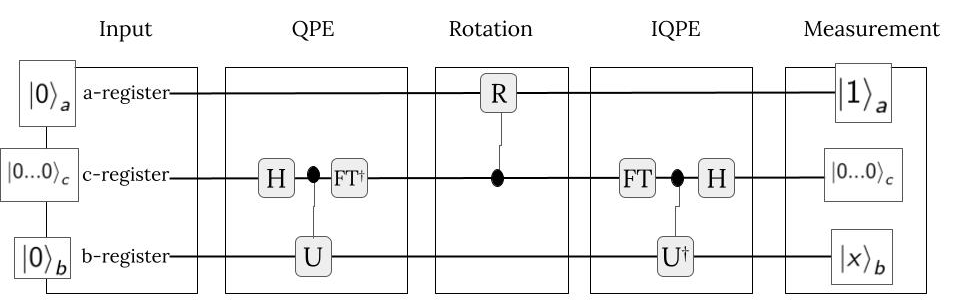
\includegraphics[width=8.5cm]{img/example_circuit_cropped.png}
    \caption{Example Circuit}
    \label{ex_circ}
\end{figure}

Now we will take a look at how the algorithm is implemented as a quantum circuit. 
Firstly, we will look at the registers of the quantum circuits. 
Then, we will describe the phases of the procedure.

\subsubsection{Registers}
Fig.~\ref{ex_circ} shows the scheme of a simple quantum circuit for the HHL algorithm.
We have three registers that describe three different sets of qubits in the quantum circuit.

The a-register contains the ancilla qubit. 
It is used for the inversion of the eigenvalues and will be explained in detail later on.

The c-register, oftentimes referred to as the clock-register, is used for the QPE part. It is related to the time (clock) of the controlled rotation of the qubits and will store the eigenvalues after performing QPE.

The b-register contains the $\vec{b}$ vector which is encoded into a quantum state $\ket{b}$. 
After the whole HHL procedure is done, the b-register will contain the solution state $\ket{x}$.



\subsubsection{Phases}
The procedure of the quantum circuit can be split into 5 phases:

\begin{itemize}
\item State preparation
\item Quantum phase estimation (QPE)
\item Inversion of eigenvalues
\item Inverse quantum phase estimation (IQPE)
\item Measurement of $\ket x$
\end{itemize}

In the state preparation phase, the vector $\vec{b}$ will be encoded into a quantum state $\ket{b}$ and the $A$ matrix will be encoded as a Hamiltonian, which is a unitary operator
$U=e^{iAt}$ into the QPE and IQPE operations.

Then, the QPE will calculate the eigenvalues and eigenvectors of the A matrix.

Afterward, we perform the inversion of the eigenvalues through rotary operations. 
These operations have a probability to fail, as they are not unitary operators.
The ancilla will detect whether the rotation was successful or not and will either collapse to $\ket0$ or $\ket1$ for failure and success.
If the rotation is not successful, the procedure has to be repeated from the beginning. 
If the rotation was successful we can continue the procedure. 
The problem is, that the qubits in the b-register and c-register are entangled. 
This means that we cannot factorize the result into a tensor product of the c-register and b-register.
As a result, we cannot convert the b-register into the $\ket 0$ / $\ket 1$ measurement basis with the desired amplitudes.
We will need to uncompute the state, thus, we have to undo all operations up until now, to unentangle the states whilst keeping the inverted eigenvalues.

This is achieved by the IQPE which undos all steps we performed in the QPE phase, leaving us with the $\ket{0...0}$ state in the c-register and the $\ket x$ state in the b-register.

Lastly, the $\ket x$ state is to be measured. As mentioned earlier, we can only read out an approximation of an expectation value $\bra x M \ket x$.

\section{The HHL Algorithm}
The next section will give a more detailed walkthrough of the HHL algorithm.
Thereby, it will go through all the 5 phases namely, state preperaration, QPE, inversion of eigenvalues, IQPE and lastly the measurement.

\subsection{State Preparation}

In total we have $n_b + n + 1$ qubits. 
In the beginning they are all initialized in their zero state as
\begin{equation}
\begin{split}
\ket{\Psi_0} &= \ket{0\dots0}_b\ \ket{0\dots0}_c\ \ket{0}_a \\
&= \ket{0}_b^{{\otimes n_b}}\ \ket{0}_c^{\otimes b}\ \ket{0}_a 
\end{split}
\end{equation}
We now have to load the vector $\vec{b}$ into the b-register. 
This is achieved by amplitude encoding. 

Todo 

insert formula here

The state $\ket b$ is then loaded into the b-register. Therefore

\begin{equation}
\ket{\Psi_1} = \ket{b}_b\ \ket{0\dots0}_c\ \ket{0}_a
\end{equation}

We have successfully encoded the $\vec{b}$ into our b-register. 
We now continue with the QPE. 

\subsection{Quantum Phase Estimation}
We will only briefly go through the specifics of the QPE and will not discuss each step in detail, as this is not the main topic of this paper. 
For further explanations refer to this paper.
As already mentioned, the QPE is a procedure to evalute an estimate of eigenvalues. 
It consists of three phases, namely the superpositions of the clock-bits via Hadamard gate, controlloed rotation via unitary U and the IQFT.
After QPE we will have an estimate of the eigenvalues of the unitary $U$. 
As we have encode $A$ as as a Hamiltonian $U = e^{iAt}$, the phase of the eigenvalue of U is proportional to the eigenvalue of $A$.
We have to define a scaled version of our eigenvalues $\lambda_j$.
\begin{equation}
\widetilde{\lambda_j} = \frac {N\lambda_jt}{2\pi}
\end{equation}
where $t$ can be choosen freely so that the scaled eigenvalues $\widetilde{\lambda_j}$ are integers.

Thus, the eigenvalues of $A$ will be stored in the c-register after QPE as
\begin{equation}
\begin{split}
\ket{\Psi_2} &= \ket{b}_b \ket{\widetilde{\lambda}}_c\ket{0}_a \\
% &=\left(-\frac{1}{\sqrt{2}} \ket{u_0} \ket{01} +\frac{1}{\sqrt{2}}  \ket{u_1} \ket{10} \right)  \ket{0}_a\\
& =\sum_{j=0}^{N-1} b_j \ket{u_j}_b \ket{\widetilde{\lambda_j}}_c \ket 0_a
\end{split}
\end{equation}
Notice, that the b-register is now a representation of the $\ket b$ state in the eigenbasis $\ket{u_j}$ of $A$.

\subsection{Inversion of the eigenvalues}
In the next step we want to invert the eigenvalues in our state. 
This is achieved by the rotation of the ancilla qubit in the a-register by the eigenvalues in the c-register.
The state of the registers after the rotation looks like this

\begin{equation}
\ket{\Psi_3} = \sum_{j=0}^{N-1} b_j \ket{u_j}_b {\ket{\widetilde{\lambda_j}}}_c \left(\sqrt{1-\frac{C^2}{\widetilde{\lambda_j^2}}}\ket{0}_a + \frac{C}{\widetilde{\lambda_j}} \ket{1}_a\right)
\end{equation}

where $C$ is a constant that should be chosen to be as large as possible to increase the success probability.
Currently, the state of the a-register can either collapse into $\ket 1$ or $\ket 0$. 
The probability of the state collapsing to $\ket 1$ is $\left|\frac C {\widetilde{\lambda_j}}\right|^2$.
If the ancilla bit collapses to $\ket 0$, the whole procedure has to be repeated from the beginning. 
As mentioned earlier this has to be done, because the rotation process is not unitary and has a probability to fail.

We assume that our rotation process was successfull and the ancilla bit collapses to $\ket 1$. 
The registers will look as such
\begin{equation}
\ket{\Psi_4}= \frac {1} {\sqrt{\sum_{j=0}^{N-1}   \left|  \frac{b_jC} {\widetilde{\lambda_j}}\right|^2   }} 
\sum_{j=0}^{N-1} b_j \ket{u_j}_b \ket{\widetilde{\lambda_j}}_c \frac{C}{\widetilde{\lambda_j}} \ket1_a
\end{equation}
Note that term in front of the sum is just a factor to normalize the state. 
Lets call this normalization factor $D$.
We see that we now have a term $\frac{C}{\widetilde{\lambda_j}}$ that represents the inverted eigenvalues. 
This term can be moved around freely as it is just a scalar and can be moved, such that it is applied to the b-register
\begin{equation}
\ket{\Psi_4}= D
\sum_{j=0}^{N-1} \frac{C}{\widetilde{\lambda_j}} b_j \ket{u_j}_b \ket{\widetilde{\lambda_j}}_c \ket1_a
\end{equation}

If we go back to our idea from the mathematical overview section, our b-register is in the same form as our solution state
\begin{equation}
\ket{x} = \sum_{i=0}^{N-1} \lambda_i^{-1} b_j\ket{u_j}\\
\end{equation}

That means our solution is already encoded in our registers. 
The problem here is, that we cannot read the solution out yet.
This has to with the states in the b-register and c-register being entangled with each other. 
That means we cannot convert the b-register into a $\ket0 / \ket 1$ measurement.
In the following we have to undo all operations to unentangle the state in the b-register and c-register, to achieve the correct result.

\subsection{Inverse Quantum Phase estimation.}
The unentangling of the registers is achieved throught the IQPE which just backtracks all calculations of the QPE.
We are left with the following state

\begin{equation}
\begin{split}
\ket{\Psi_5} &= \frac {1} {\sqrt{\sum_{j=0}^{N-1} \left| \frac{b_jC} {\lambda_j}\right|^2}}
\sum_{j=0}^{N-1}\frac{ C}{\lambda_j}   b_j \ket{u_j}_b \ket{0}_c^{\otimes n} \ket{1}_a\\
&= \frac {C} {\sqrt{\sum_{j=0}^{2^{n_b}-1} \left| \frac{b_jC} {\lambda_j}\right|^2}}
\ket{x}_b \ket{0}^{\otimes n}_c \ket{1}_a
\end{split}
\end{equation}

The a-register is untouched and still hold the $\ket 1$ state as before. 
The c-register however is reset to the zero state $\ket{0}^{\otimes n}_c$ as in the beginning of the process. 
It is now unentangled from the b-register.
The b-register now contains the solution $\ket x$ after the uncomputation and can be measuremed correctly.

We can furthermore simplify the term as we assume that  $C$ is real and that the eigenvectors $\ket{u_i}$, and the $\ket b$ state are normalized.
Then we can simplify to 

\begin{equation}
\begin{split}
\ket{\Psi_5} &= \frac {1} {\sqrt{\sum_{j=0}^{N-1} \left| \frac{b_j} {\lambda_j}\right|^2}}
\ket{x}_b \ket{0}^{\otimes n}_c \ket{1}_a\\
&= \ket{x}_b \ket{0}^{\otimes n}_c \ket{1}_a
\end{split}
\end{equation}

We can now  read out the result $\ket x$ in the b-register.

\subsection{Measurement}
As mentioned earlier, we cannot obtain the whole solution for the $\vec x$ as reading out all the entries would cost us $\mathcal{O}(N)$ steps.
This would ommit our speedup of $\mathcal{O}(log N)$. 
That means that by measuring, we will only obtain an estimate of specific features of $\ket x$.
Using a linear operator $M$ we can perform various measurements on $\ket x$ by calculating the inner product as such
\begin{equation}
    \bra x M \ket x
\end{equation}
With this we can extract various statistical features of $\ket x$ like the norm of the vector, the average of the weight of the components, moments, probability distributions, localization and concentration in specific regions, etc.



























\section{Easy Example}

In this section, we will go through an easy numerical example of the HHL algorithm.
The quantum circuit that we will be using contains 4 qubits.
The scheme of the quantum circuit is shown Fig. 2.
Firstly, we will have to set some preliminary values to make our calculations easier. 
Then, we will go through all 5 phases of the HHL algorithm. 

\subsection{Preliminaries}
We are given the matrix $A$ and the vector $\vec{b}$ as such
\begin{equation}
   A = \begin{pmatrix} 1 & -\frac{1}{3}\\ -\frac{1}{3} & 1\\ \end{pmatrix}
\end{equation}

\begin{equation}
    \vec{b} = \begin{pmatrix} 0 \\ 1\\ \end{pmatrix}
\end{equation}

If we calculate the solution classically we will obtain the solution vector 
\begin{equation}
\vec{x} = \begin{pmatrix} \frac{3}{8}\\ \frac{9}{8}\\ \end{pmatrix}
\end{equation}

As we already discussed, the HHL algorithm doesn't solve for the whole solution vector $\vec{x}$, as we are only interested in some estimation value $\ket x M \ket x$.
To compare the results of both methods we will take the probability ratio of the entries of our solution vector $\vec x$ and $\ket x$.
To calculate the probability ratio, we have to divide by the square of each entry of $\vec{x}$.
Thus, we obtain a ratio of
\begin{equation}
    \frac{ |x_0|^2}{ |x_1|^2}= \frac{\frac{9}{64}}{\frac{81}{64}} = \frac{1}{9}
\end{equation}
where $x_0$ and $x_1$ are the entries of $\vec x$.

To make simplify our calculations, we will cheat by determining the eigenvectors and eigenvalues beforehand.
Normally, the QPE would calculate these numbers, but as the main focus of this paper is the HHL algorithm, we will not go through each step of the QPE.
For a more thorough walkthrough, please refer to the this example \cite{step}.
The eigenvectors of the matrix $A$ are
\begin{equation}
\vec{u_0} = \begin{pmatrix} \frac{-1}{\sqrt{2}}\\ \frac{-1}{\sqrt{2}}\\ \end{pmatrix}\\
\end{equation}

\begin{equation}
\vec{u_1} = \begin{pmatrix} \frac{-1}{\sqrt{2}}\\ \frac{1}{\sqrt{2}}\\ \end{pmatrix}
\end{equation}

These can be represented through amplitude encoding in our quantum circuit
\begin{equation}
\ket{u_0} = \frac{-1}{\sqrt{2}}\ket{0} + \frac{-1}{\sqrt{2}}\ket{1}
\end{equation}

\begin{equation}
\ket{u_1}= \frac{-1}{\sqrt{2}}\ket{0} + \frac{1}{\sqrt{2}}\ket{1} 
\end{equation}

Additionally, we also have to determine the eigenvalues. The eigenvalues $\lambda_j$ of the matrix $A$ are
\begin{equation}
\lambda_0 = \frac{2}{3}
\end{equation}

\begin{equation}
\lambda_1 = \frac{4}{3}
\end{equation}

We then have to encode the eigenvalues into a quantum state $\ket{\widetilde{\lambda_j}}$.
In the encoding scheme $\widetilde{\lambda_j} = N_q\lambda_jt/2\pi)$, we can freely choose a $t$ such that we obtain an easy encoding of the eigenvalues. 
Here $N_q$ refers to the number of qubits in our system, which means $N_q = 4$.
If we choose $t = 3\pi/4$, then we will obtain
\begin{equation}
\widetilde{\lambda_0} =\frac{4*\frac{2}{3}*\frac{3\pi}{4}}{2 \pi} =\frac{4*2*3\pi}{3*4* 2 \pi} = 1
\end{equation}
\begin{equation}
\widetilde{\lambda_1} =\frac{4*\frac{4}{3}*\frac{3\pi}{4}}{2 \pi} =\frac{4*4*3\pi}{3*4* 2 \pi} = 2
\end{equation}
which can be encoded through basis encoding into the quantum circuit.
Thus, we are left with these states
\begin{equation}
\ket{\widetilde{\lambda_0}} = \ket{01}
\end{equation}
\begin{equation}
\ket{\widetilde{\lambda_1}} = \ket{10}
\end{equation}

Now we can start with our procedure.

\subsection{Numerical walkthrough}

In Fig.~\ref{ex_circ_numerical} we can see that we have 1 qubit each for the a-register and b-register, corresponding to the ancilla bit and the intput $\vec b$.
The c-register has 2 qubits, as we have to store the two eigenvalues $\lambda_1$, $\lambda_2$ we calculated just now.
Our starting state looks like this
\begin{equation}
\ket{\Psi_0} = \ket{0}_b\ \ket{00}_c\ \ket{0}_a = \ket{0000}
\end{equation}
as all registers are initalized with the zero state.


\begin{figure}
    \centering
    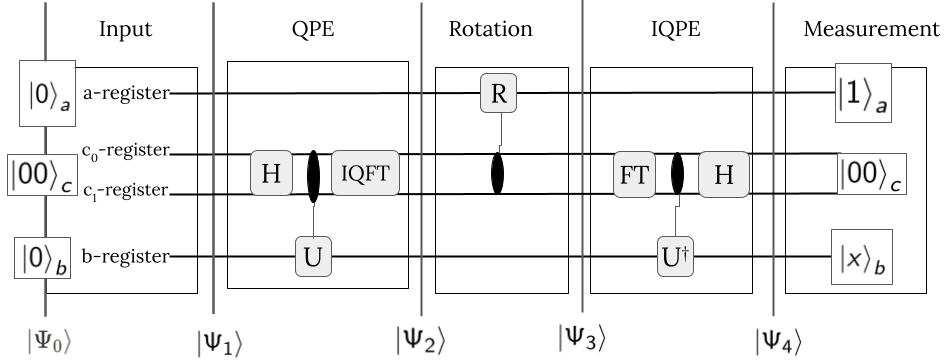
\includegraphics[width=8.5cm]{img/example_circuit_4_qubit_cropped.png}
    \caption{4-Qubit Circuit}
    \label{ex_circ_numerical}
\end{figure}




\subsubsection{State preparation}
    Here we have to encode our vector $\vec{b}$ into the quantum state $\ket{b}$, using amplitude encoding.
    Thus, we obtain
    \begin{equation}
    \vec{b} = \begin{pmatrix} 0\\ 1\\ \end{pmatrix}
    \Leftrightarrow \ket{b} = 0 \ket{0} + 1 \ket{1} = \ket{1} 
    \end{equation}
    which makes sense as the $\ket 1$ state is defined as the $\begin{pmatrix} 0\\ 1\\ \end{pmatrix}$ vector.
    Loading $\ket b$ into our quantum circuit, our state looks like this
    \begin{equation}
    \ket{\Psi_1} = \ket{1}_b\ \ket{00}_c\ \ket{0}_a = \ket{1000}
    \end{equation}

\subsubsection{Quantum Phase Estimation}
    The QPE determines the eigenvalues $\lambda_j$ of the $A$ matrix. 
    These are stored in the c-register. 
    The b-register now stores $\ket b$ in the eigenbasis state of $A$ leading us to the following state
    \begin{equation}
    \ket{\Psi_2} = \ket{b}_b \ket{\widetilde{\lambda}}_c\ket{0}_a
    \end{equation}
    \begin{equation}
    \ket{\Psi_2} =\left(-\frac{1}{\sqrt{2}} \ket{u_0}_b \ket{01}_c +\frac{1}{\sqrt{2}} \ket{u_1}_b \ket{10}_c \right)  \ket{0}_a
    \end{equation}


\subsubsection{Inversion of the eigenvalues}
    Now we have to invert the eigenvalues. 
    This is achieved by rotating the a-registers by the eigenvalues in the c-register.
    This leaves us in this state

    \begin{equation}
     \begin{split}
    \ket{\Psi_3} =& \sum_{j=0}^{2^{1}-1} b_j \ket{u_j} \ket{\widetilde{\lambda}_j} \left(\sqrt{1-\frac{C^2}{\widetilde{\lambda}_j^2}}\ket{0} + \frac{C}{\widetilde{\lambda}_j} \ket{1}\right) \\
    =&-\frac{1}{\sqrt{2}} \ket{u_0} \ket{01}\left(\sqrt{1-\frac{1}{1^2}}\ket{0} + \frac{1}{1} \ket{1}\right) \\
    &+\frac{1}{\sqrt{2}}  \ket{u_1} \ket{10} \left(\sqrt{1-\frac{1}{2^2}}\ket{0} + \frac{1}{2} \ket{1}\right)
     \end{split}
    \end{equation}

    We assume that our rotation was successful and we measure $\ket{1}$ in the ancilla qubit, then
    

    \begin{equation}
    \begin{split}
    \ket{\Psi_3} &=\sqrt{\frac{8}{5}}\left(\frac {1} {\widetilde{\lambda_0}} *-\frac{1}{\sqrt{2}} \ket{u_0}_b\ket{01}_c +\frac{1}{\widetilde{\lambda_1}}*\frac{1}{\sqrt{2}} \ket{u_1}_b\ket{10}_c\right)\ket{1}_a \\
    &=\sqrt{\frac{8}{5}}\left(-\frac{1}{\sqrt{2}} \ket{u_0}_b\ket{01}_c +\frac{1}{2\sqrt{2}} \ket{u_1}_b\ket{10}_c\right)\ket{1}_a 
    \end{split}
    \end{equation}

    Note that the b-register and c-register are entangled. We now have to unentangle the registers.

\subsection{Inverse Quantum Phase Estimation}
    We now backtrack all the steps in the QPE through IQPE.
    The c-register is reset to the zero state again and the b-register contains our solution state $\ket x$.
    The state of the circuit looks like this
    \begin{equation}
    \ket{\Psi_4}= \ket{x}_b \ket{00}_c \ket{1}_a 
    \end{equation}
    \begin{equation}
    \ket{\Psi_4}=\frac{1}{2}\sqrt{\frac{2}{5}}  \left(\ket{0} +3 \ket{1} \right) \ket{00}_b \ket{1}_a
    \end{equation}

\subsection{Measurment}
    Now we have to measure the solution state $\ket x$.
    In the beginning, we decided to take the probability ratio as our solution. 
    To get the probability of $\ket{u_0}$ and $\ket{u_1}$ we have to square their coefficients
\begin{equation}
\begin{split}
c_0&=\left|\frac{1}{2}\sqrt{\frac{2}{5}}*1\right|^2 = \frac{1}{20}\\
c_1&=\left|\frac{1}{2}\sqrt{\frac{2}{5}}*3\right|^2 = \frac{9}{20}
\end{split}
\end{equation}

As expected our ratio is 
\begin{equation}
 \frac{\frac{1}{20}}{ \frac{9}{20} } = \frac 1 9
\end{equation}


\section{Evaluation}

\begin{comment}
look at gauß verfahren 
not fastest
look at same constraints 
conjugate gradient descent much faster with similiar requirements
only interested in estimate of $\vec{x}^\dagger M \vec x$
this runs in $ \mathcal{O}(\kappa s log{\left(\frac 1 \epsilon\right)} N ) $
where 
\end{comment}

In this section, we evaluate the performance of the HHL algorithm and will shortly look at resource requirements.

The most commonly known method to solve a system of linear equations is Gaussian Elimination. 
The time complexity of the Gaussian is $\mathcal{O} (N^3)$, being drastically slower than other classical methods.
As we are only interested in an estimate of an expectation value $\bra x M \ket x$, we can take a look at similar classical methods, considering the constraints.

In the following we will compare the HHL algorithm, to the classical conjugate gradient descent algorithm, focusing on time complexity and other factors that impact its efficiency \cite{hhl}.

\subsection{Conjugate Gradient Descent}
The classical conjugate gradient descent algorithm is a very common method for solving linear systems of equations. 
It uses the conjugate direction method, which can locate the minimum of a function. 
By iteratively looking for solution vectors, the procedure converges toward the solution of the linear system.
This will provide us with a suitable benchmark for analyzing the efficiency of the HHL algorithm, since it also estimates a solution vector.
Not only is it one of the fastest classical algorithms, but also has a very similar constraint set and calculates similar results (eg. $\vec{x}^\dagger M \vec x$).

\subsection{Comparison of Time Complexity }
\begin{table}[htbp]
    \caption{Time complexity comparison}
    \begin{center}
    \begin{tabular}{|c|c|}
    \hline
    \textbf{Conjugate Gradient Descent} & \textbf{HHL Algorithm} \\
    \hline
    $\mathcal{O}(\kappa s \log\left(\frac{1}{\epsilon}\right) N)$  &  $\mathcal{O}\left(\frac{\kappa^2s^2}{\epsilon}\log N\right)$\\
    \hline
    $\Rightarrow \mathcal{O} (N)$ & $\Rightarrow \mathcal{O} (log(N))$\\ 
    \hline
    \end{tabular}
    \end{center}
\end{table}

As shown in the table, the HHL algorithm offers an exponential improvement compared to the conjugate gradient descent method.
Conjugate gradient descent achieves a time complexity of $\mathcal{O}(N)$, whereas the HHL algorithm runs in $\mathcal{O}(log(N))$.

Now we will take a more detailed look a the other factors involved in the time complexity, where:
\begin{itemize}
    \item $\epsilon$ is the accuracy
    \item $s$ is the s-sparseness
    \item $\kappa$ is the condition number
\end{itemize}

Firstly, $\epsilon$ describes the accuracy of our desired solution.
The sparseness $s$ describes to number of non-zero entries per row
(e.g. a 2-sparse matrix only contains 2 non-zero entries per row).
The condition number $\kappa$ describes how sensitive the output of a function is at the error of the input.
That means, a function is well conditioned if the output of a function does not change by much if the errors in the input are big.
These two factors are related to the QPE phase, since a unitary $e^{iAt}$ has to be generated. 
This step heavily relies on the sparsity $s$ and conditioning $\kappa$ of the matrix $A$ to be performed efficiently.
If not, this process would grow $\mathcal{O}(N^c)$ for some constant $c$.
Again, this would omit our speedup of $\mathcal{O}(log(N))$.

We can observe, that the sparsity $s$ and condition number $\kappa$ are quadratic in the HHL algorithm, whereas in the conjugate gradient descent algorithm, both factors operate linearly.
Furthermore, the accuracy $\epsilon$ is exponentially worse in the HHL algorithm. 
Thus, in terms of sparsity, accuracy and condition number, the HHL algorithm has a worse runtime than the conjugate gradient descent algorithm.
If these prefactors were not worse than in the classical solution, this would have bizarre implications. 
We are able to show that if the dependency of these factors is better or equal as in the classical solution, we could solve \textit{NP-Complete} problems exponentially faster on quantum computers, which seems unlikely.
All in all, these constraints are important to consider when choosing applications, as they have a great effect on the runtime \cite{fineprint}.


\subsection{Resource requirements}
The resource requirements to implement the HHL algorithm are substantial.
Looking at the structure of the algorithm it has a very similar structure to Shor's algorithm, having QPE as its main routine.
Hence, we can use Shor's procedure as a lower bound to estimate the resource requirements.
Shor's algorithm for 2048 RSA, needs roughly 4000 logical qubits to work properly. 
To compensate for error correction and other quantum effects in the circuit, this would take millions of qubits. 
Although, these numbers have dropped many times over the past couple of years.

\section{Applications and Variations} 
In this section we will take a look at the future outlooks of the HHL algorithm and summarize our results.
We will explore potential applications given the constraints set of the HHL algorithm.
Then we will delve into different variations and optimizations which can improve the performance. 
Lastly, we will discuss some broad perspective, that the HHL algorithm offers in the field of quantum computing. 

\subsection{Applications}
The main problem wih the HHL algorithm is, that it does not output the full solution vector, but rather the solution state $\ket x$.
Not to be forgotten is, that the matrix $A$ has to be sparse for the HHL algorithm to work efficiently.
But in some cases these constraints are not a problem and can therefore be solved by the HHL algorithm.
We will now discuss some examples that utilize the algorithm. 

    \subsubsection{Analyzing Large Sparse Electrical Networks}
    The HHL algorithm can be applied to analyze large sparse electrical networks, where we are interested in an estimate of a specific feature.
    Electrical networks consist of vast numbers of interconnected components, like generators, transformers, transmission lines, etc. 
    Though, these networks have a high number of components, they have a relative low amount of connections between the each other.
    Thus, systems can be modeled as a graph which correspond to large sparse matrices.
    By being able to calculate the inverse of a matrix $A^{-1}$ efficienly, we can deduct many network properties, such as resistance. 
    This can help us to further optimize the electrical powersystem.
    Conventionally, we would have to rely on iterative algorithms, which are as we saw earlier, exponentially slower in this specific case \cite{electrical_networks}.
    
    \subsubsection{Machine Learning (Least-Square Estimation)}
    In the field of machine learning the HHL algorithm can also massively improve calculations. 
    The HHL algorithm also plays a significant role in the field of machine learning, as it can improve computational intensive calculations.
    For example in least-square estimation, the HHL algorithm can be used to determine estimates of inverse matrices. 
    This can be very helpful in data fitting tasks, enabling efficient parameter estimation and model optimization \cite{data_fitting}.
    
All in all, finding more applications for the HHL algorithm is crucial, given its specific constraints and promising capabilities.

\subsection{Variations and Optimizations}
Current research and developments have been able to find variations and optimizations to the HHL algorithm.
These changes have brought more efficient ways to perform the HHL algorithm and expand its applicability.
We will now discuss some examples of improvements done to the HHL algorithm.

    \subsubsection{Ancilla Bit Requirement} 
    Certain variants allow the HHL algorithm to operate without an ancilla bit.
    This eliminates the probability of failure in the rotation step of the eigenvalues, which leads to a faster walkthrough, as one must not repeat the process mutliple times at failure.
    Additionally, this increases the reliability of the algorithm \cite{without_ancilla}.

    \subsubsection{QRAM}
    Quantum Random Access Memory (QRAM) is the quantum computer equivalent of the classical ram in a computer.
    It enables the the quantum computer to directly access quantum states for computation witheut having to encode the input. 
    This would provide us with a very efficient way to load our state $\ket b$ into our quantum circuit \cite{qram}.

Exploring these variations and identifying novel optimizations can contribute to the advancement and practical implementation of the HHL algorithm.


\subsection{IT Security}
Although, the HHL algorithm is primarily designed for solving linear system, there are potential applications in the field of IT security.
We will now discuss some examples how one could utilize the algorithm IT security.

    \subsubsection{Solving Large-scale Linear Systems}
    The HHL algorithm can contribute to the efficient calculation of large-scale linear systems.
    These are required in many IT security protocols, such as secure multi-party computation or zero-knowledge proofs. 

    Multi-party computation is as protocol that enables multiple different machines to computer a function, whilst not revealing their data to each other. 
    The protocol achieves this by using linear systems as a subroutine to achieve secrecy.

    Zero knowledge proofs are methods that enable a party to demonstrate certain features to another party without revealing any other information except the validity of that feature.
    This can be useful to verify your identity without giving out any personal data.
    Oftentimes these zero knowledge proofs can be modeled in linear systems, which then can be processed by the HHL algorithm.

    \subsubsection{Pattern recognition for fraud dection}
    Pattern recognition for fraud detection is also a possible application for the HHL algorithm.
    Again, this plays in the field of machine learning. 
    Here various big data analysis methods are used to detect fraudulant activites, which can be accelerated by the HHL algorithm.









\section{Conclusion}

In conclusion, the HHL algorithm offers a significant improvement over its classical counterpart, considering its constraints.
Sparsity, a low condition number and error are needed for the HHL algorithm to work efficiently.
Additionally, ways to load the input vector faster, for example with Qram, are needed. 
In the end, we observed, that the sparsity and conditioning of the problem matrices $A$, have a comparable dependency on the runtime, but the error dependency is exponentially worse. 

Despite these constraints, the HHL algorithm has made significant contributions, especially in the field of quantum machine learning. 
Since there are no ground-breaking applications so far, the Shor's algorithm, that has the ability to break the RSA encryption, further use cases need to be found.
Nonetheless, the ongoing discussions and research on the algorithm enable us to discover new optimizations and applications.
The advances in quantum algorithms, including the HHL algorithm, have laid the foundation for future developments in the field.
Because of the generality of the HHL algorithm, it has the potential to be used as a subroutine in various domains.

While experiments have demonstrated that the HHL algorithm works on small quantum computers with high fidelity, 
more advancements, as better error correction and scaling are needed to unlock the full potential of quantum computing.





\begin{thebibliography}{00}
\bibitem{a1} A. Harrow, A. Hassidim, and S. Lloyd, "Quantum algorithm for linear systems of equations," Phys. Rev. Lett. 103, 150502, 2009
\bibitem{citekey} H. Morrell Jr, A. Zaman, H. Wong, "Step-by-Step HHL Algorithm Walkthrough to Enhance the Understanding of Critical Quantum Computing Concepts", 2021
\bibitem{citekey} D. Dervovic, M. Herbster, P. Mountney, S. Severini, N. Usher, L. Wossnig, "Quantum linear systems algorithms: a primer", 2018
\bibitem{citekey} A. Childs, R. Kothari, R. Somma, "Quantum algorithm for systems of linear equations with exponentially improved dependence on precision", SIAM Journal on Computing 46, 1920-1950, 2017
\bibitem{citekey} D. Babukhin, Harrow-Hassidim-Lloyd algorithm without ancilla postselection, 2022
\bibitem{citekey} N. Wiebe, D. Braun, S. Lloyd, Quantum Data Fitting, Phys. Rev. Lett. 109, 050505, 2012
\bibitem{citekey} S. Aaronson, "Read the fine print",  Nature Phys 11, 291-293, 2015 
\bibitem{citekey} G. Wang, Efficient Quantum Algorithms for Analyzing Large Sparse Electrical Networks, Quantum Information \& Computation 17 (11 \& 12): 987-1026, 2017 
\bibitem{citekey}

\end{thebibliography}



\begin{comment}
    HHL-2009: 
    step by step: 
    primer: https://arxiv.org/abs/1802.08227
    exponential imprved dependencs on precision: https://arxiv.org/abs/1511.02306
    without ancilla: https://arxiv.org/abs/2208.02200
    data fitting:
    fineprint: https://inspirehep.net/literature/1834407
    large electrical networks: https://arxiv.org/abs/1311.1851
    qiskit example: https://learn.qiskit.org/course/ch-applications/solving-linear-systems-of-equations-using-hhl-and-its-qiskit-implementation#example1
\end{comment}

%
\end{document}

